\documentclass[aspectratio=169]{beamer}

% Language setup
\usepackage[magyar]{babel} % Babel for Hungarian
\usepackage[T1]{fontenc} % Output character encoding
\usepackage[utf8]{inputenc} % Input character encoding
\selectlanguage{magyar}

% Beamer styling setup
\usetheme{Boadilla}
\usecolortheme{default}
%\setbeamercolor{titlelike}{parent=structure,bg=gray!15}
\setbeamertemplate{navigation symbols}{}
\setbeamertemplate{caption}[numbered]
%

% Spacing setup
\setlength{\parindent}{0pt} % No paragraph indenting
\setlength{\parskip}{5pt} % Set spacing between paragraphs
\frenchspacing
\newcommand{\mkspace}{\vspace{19pt}}
\newcommand{\rmspace}{\vspace{-19pt}}
\newcommand{\emptyline}{\vspace{\baselineskip}}
%

% Dependency setup
\usepackage{tikz}
\usetikzlibrary{decorations.markings}
\usetikzlibrary{calc}
%

% Style setup
\usepackage{caption}
\captionsetup{format=plain, font=scriptsize, labelformat=empty}
%


% Notation setup
\usepackage{physics} % Braket notation

\author{Nemkin Viktória}
\institute{Konzulens: dr. Friedl Katalin}
\title{Kvantumséták szimulációja klasszikus számítógépen}
\subtitle{TDK (2021)}
\date{}

\begin{document}

\frame{\titlepage}

\begin{frame}
  \frametitle{Gráfbolyongások}
  \begin{itemize}
    \item Véletlen séta a gráf csúcsain (speciális Markov-lánc).
    \item Klasszikusan:
    \begin{itemize}
        \item Google kereső: PageRank
        \item Közelítő algoritmusok: SAT megoldó, részgráf keresése
    \end{itemize}
    \item Klasszikusan
        \item Véletlen nélkül kezelhetetlen problémára: PageRank
        \item Gyorsítani nem-közelítő algot: SAT megoldó, részgráf kereső
    \item Kvantum gráfbolyongás: Próbáljuk meg kvantumosan!
    \item Ki fog jönni, hogy teljesen más mint a klasszikus, gyorsabban bejárja (gyök(N) vs N) és másképp is viselkedik.
    \item Kvantum párhuzamosság kihasználása.
    \item Destruktív / konstruktív interferencia az egyes lépések között.
    \item Korszerű, nem lezárt, tudományos vizsgálatok homlokterében.
  \end{itemize}

  \textbf{Gráfbolyongás}
  \begin{itemize}
    \item Irányított, élsúlyozott gráf
    \item Csúcsok bejárása
    \item Minden lépésben: kimenő élek súlya szerint választunk
  \end{itemize}
  \pause
  \textbf{Kvantum gráfbolyongás}
  \begin{itemize}
    \item Véletlen választás: kvantumosan
    \item Speciális eset: kimenő fokszám = 2 $\rightarrow$ érme feldobás
  \end{itemize}
\end{frame}

\begin{frame}
  \frametitle{Kvantumérme}
  \textbf{Kvantumbit}
  \begin{itemize}
    \item Lehet $\ket{0}$, $\ket{1}$ vagy $c_0\ket{0} + c_1\ket{1}$ (szuperpozíció)
          \begin{itemize}
            \item 2 dimenziós vektor: $\begin{pmatrix} c_0 \\ c_1 \end{pmatrix}$
            \item $\ket{0} = \begin{pmatrix} 1 \\ 0\end{pmatrix}$, $\ket{1} = \begin{pmatrix} 0 \\ 1\end{pmatrix}$
          \end{itemize}
          \pause
    \item Megkötések:
          \begin{itemize}
            \item Koordináták komplexek
            \item Egység hosszú: $|c_0|^2 + |c_1|^2 = 1$
          \end{itemize}
          \pause
    \item Mérés eredménye: $\ket{0}$ vagy $\ket{1}$
          \begin{itemize}
            \item $P(\ket{0}) = |c_0|^2$
            \item $P(\ket{1}) = |c_1|^2$
          \end{itemize}
  \end{itemize}
\end{frame}

\begin{frame}
  \frametitle{Kvantumérme}

  \textbf{Hadamard-kapu} (mátrix)
  \[\begin{pmatrix} c_0' \\ c_1'
    \end{pmatrix} = \begin{pmatrix} \frac{1}{\sqrt{2}} & \frac{1}{\sqrt{2}}
      \\ \frac{1}{\sqrt{2}} & -\frac{1}{\sqrt{2}}\end{pmatrix} \cdot
    \begin{pmatrix} c_0 \\ c_1 \end{pmatrix}\]

  \pause
  \textbf{Kvantumérme}\\
  \begin{itemize}
    \item Érme $=$ kvantumbit
    \item Érme feldobása $=$ Hadamard-mátrixszal szorzás
  \end{itemize}
\end{frame}

\begin{frame}
  \frametitle{Kvantumérme}

  Kiindulás:

  \[\ket{0} = \begin{pmatrix} 1 \\ 0 \end{pmatrix}\]
  \pause
  1. feldobás után:

  \[\begin{pmatrix} \frac{1}{\sqrt{2}} & \frac{1}{\sqrt{2}}
      \\ \frac{1}{\sqrt{2}} & -\frac{1}{\sqrt{2}}\end{pmatrix} \cdot
    \begin{pmatrix} 1 \\ 0 \end{pmatrix} = \begin{pmatrix}
      \frac{1}{\sqrt{2}} \\ \frac{1}{\sqrt{2}}
    \end{pmatrix} \]
  \pause
  $\rightarrow$ Ha megmérnénk:

  \[P(\ket{0}) = P(\ket{1}) = \left(\frac{1}{\sqrt{2}} \right)^2 = \frac{1}{2}\]


\end{frame}

\begin{frame}
  \frametitle{Kvantumérme}

  Majd:

  \[\begin{pmatrix}
      \frac{1}{\sqrt{2}} \\ \frac{1}{\sqrt{2}}
    \end{pmatrix}\]
  \pause
  2. feldobás után:

  \[\begin{pmatrix} \frac{1}{\sqrt{2}} & \frac{1}{\sqrt{2}}
      \\ \frac{1}{\sqrt{2}} & -\frac{1}{\sqrt{2}}\end{pmatrix} \cdot
    \begin{pmatrix} \frac{1}{\sqrt{2}} \\ \frac{1}{\sqrt{2}} \end{pmatrix} = \begin{pmatrix}
      1 \\ 0
    \end{pmatrix} \]
  \pause
  $\rightarrow$ Ha megmérnénk:

  \[P(\ket{0}) = 1, P(\ket{1}) = 0\]


\end{frame}

\begin{frame}
  \frametitle{Egyenesen bolyongás}

  \tikzset{axis line style/.style={thin, gray, -stealth}}

  \newcommand*{\TickSize}{2pt}%

  \begin{center}
    \begin{tikzpicture}

      \draw [axis line style] (-6.5,0) -- (6.5,0);

      \foreach \x in {-6,-5,...,6} {%
          \draw ($(\x,0) + (0,-\TickSize)$) -- ($(\x,0) + (0,\TickSize)$)
          node [below=0.1cm] {$\x$};
        }

      \draw[draw, fill=black] (0,0) circle (0.05);

      \draw[->] (0.1,0.5) -- (1,0.5) node [above=0.1cm] {$\ket{1}$};
      \draw[->] (-0.1,0.5) -- (-1,0.5) node [above=0.1cm] {$\ket{0}$};
    \end{tikzpicture}


  \end{center}
  Érme szuperpozícióban lesz $\rightarrow$ ,,egyszerre'' megyünk mindkét irányba.

  \pause
  $\rightarrow$ Sok lépés után: mi a pozíció eloszlása?

\end{frame}

\begin{frame}
  \frametitle{Egyenesen bolyongás}
  \begin{figure}[H]
    \centering
    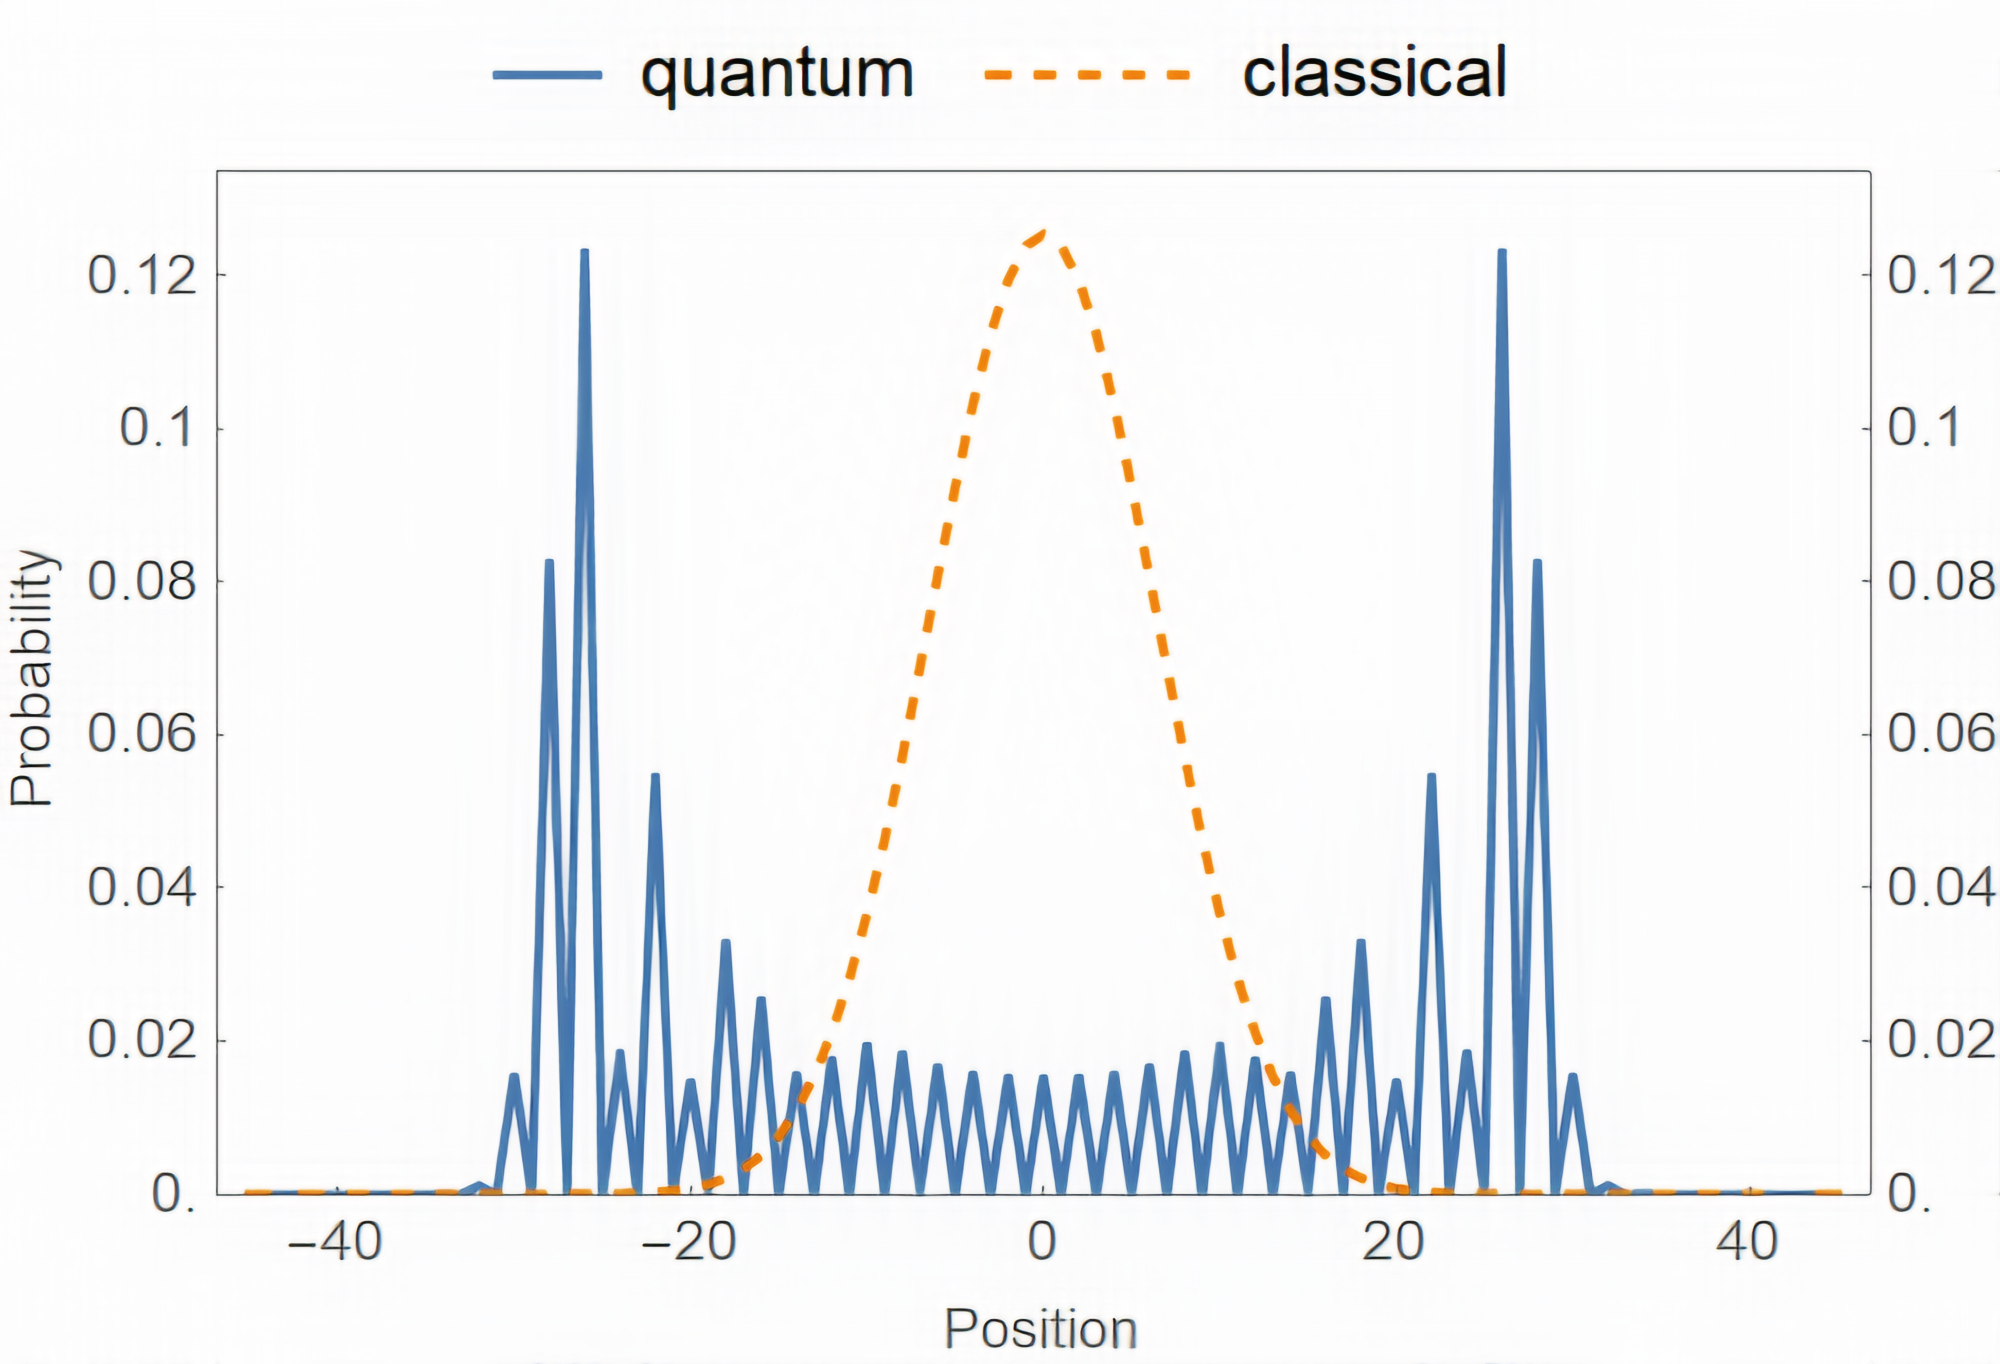
\includegraphics[width=0.6\linewidth]{./figures/teve.png}
  \end{figure}
\end{frame}

\begin{frame}
  \frametitle{TDK munka}
  \begin{itemize}
    \item Gráfbolyongási szimulációs keretrendszer Pythonban
    \begin{itemize}
      \item Kezdetben: Szomszédossági mátrix
      \begin{itemize}
        \item Nehézségek: memóriaigény, lassú iteráció az ötleteken
      \end{itemize}
      \item Megoldás: Szomszédossági orákulum, Nevesített részgráfok kompozitjai
      \item Latex report generálása
    \end{itemize}
    \item Klasszikus szimulációk
    \item Kvantum szimulációk
    \item Matematikai eredmények: 2 tétel kimondása, bizonyítása (általánosítások)
    \item Gyakorlati eredmények: Eloszlások képei, visszatérés, ballisztikus viselkedés
  \end{itemize}
\end{frame}

\begin{frame}{Klasszikus séták}
    \begin{itemize}
        \item Markov-láncok megfelelői
        \item Gráf csúcsai = val.vál. értékek
        \item Gráf szomszédossági mátrixa = átmeneti valószínűségi mátrix
        \item Hitting time, mixing time
    \end{itemize}
\end{frame}

\begin{frame}{Kvantum posztulátumok}
\begin{itemize}
\item Qubit
\item Evolúció
\item Mérés
\item Regiszer
\end{itemize}
\end{frame}

\begin{frame}
  \frametitle{Szimuláció: Egyenesen bolyongás}

  \begin{columns}[onlytextwidth]
    \begin{column}{.5\textwidth}
      \begin{figure}
        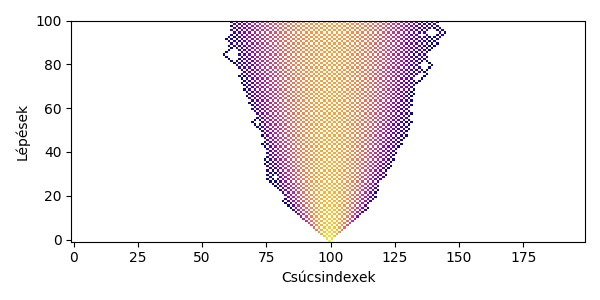
\includegraphics[width=\textwidth]{./figures/classical_simulation_short.jpg}
        \caption{\hspace{0.71cm}Klasszikus bolyongás}
      \end{figure}
    \end{column}
    \hfill
    \begin{column}{.5\textwidth}
      \begin{figure}
        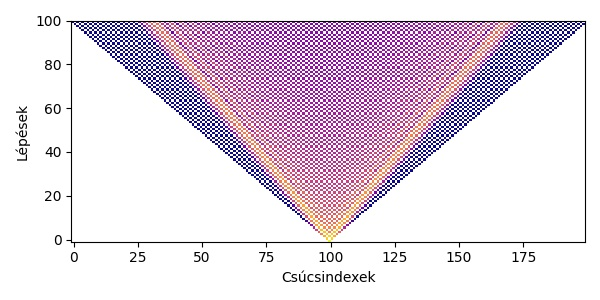
\includegraphics[width=\textwidth]{./figures/quantum_simulation_short.jpg}
        \caption{\hspace{0.73cm}Kvantum bolyongás}
      \end{figure}
    \end{column}
  \end{columns}
\end{frame}

\begin{frame}
  \frametitle{Szakaszon bolyongás}

  \begin{columns}[onlytextwidth]
    \begin{column}{.25\textwidth}
    \end{column}
    \begin{column}{.25\textwidth}
      \begin{figure}
        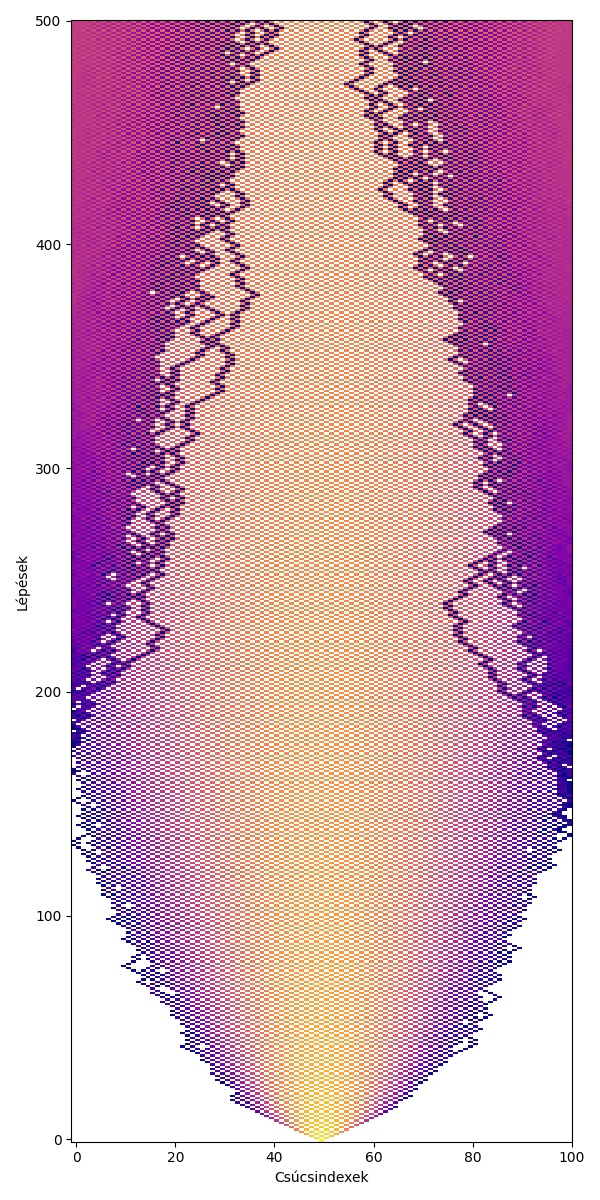
\includegraphics[width=0.9\textwidth]{./figures/classical_simulation_long.jpg}
        \caption{\hspace{0.28cm}Klasszikus bolyongás}
      \end{figure}
    \end{column}
    \begin{column}{.25\textwidth}
      \begin{figure}
        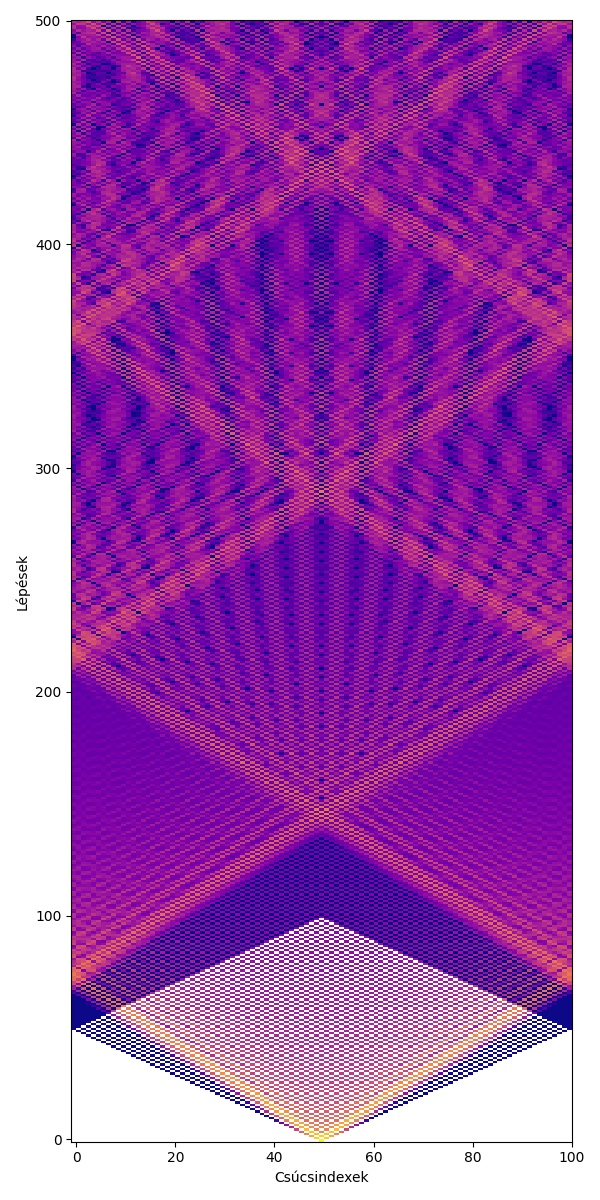
\includegraphics[width=0.9\textwidth]{./figures/quantum_simulation_long.jpg}
        \caption{\hspace{0.28cm}Kvantum bolyongás}
      \end{figure}
    \end{column}
    \begin{column}{.25\textwidth}
    \end{column}
  \end{columns}
\end{frame}


\end{document}
